\documentclass[12pt]{report}
\usepackage[utf8]{inputenc}
\usepackage[russian]{babel}
%\usepackage[14pt]{extsizes}
\usepackage{listings}
\usepackage{graphicx}
\usepackage{amsmath,amsfonts,amssymb,amsthm,mathtools} 
\usepackage{pgfplots}
\usepackage{filecontents}
\usepackage{indentfirst}
\usepackage{eucal}
\usepackage{amsmath}
\usepackage{enumitem}
\frenchspacing

\usepackage{indentfirst} % Красная строка


%\usetikzlibrary{datavisualization}
%\usetikzlibrary{datavisualization.formats.functions}

\usepackage{amsmath}


% Для листинга кода:
\lstset{ %
language=caml,                 % выбор языка для подсветки (здесь это С)
basicstyle=\small\sffamily, % размер и начертание шрифта для подсветки кода
numbers=left,               % где поставить нумерацию строк (слева\справа)
numberstyle=\tiny,           % размер шрифта для номеров строк
stepnumber=1,                   % размер шага между двумя номерами строк
numbersep=5pt,                % как далеко отстоят номера строк от подсвечиваемого кода
showspaces=false,            % показывать или нет пробелы специальными отступами
showstringspaces=false,      % показывать или нет пробелы в строках
showtabs=false,             % показывать или нет табуляцию в строках
frame=single,              % рисовать рамку вокруг кода
tabsize=2,                 % размер табуляции по умолчанию равен 2 пробелам
captionpos=t,              % позиция заголовка вверху [t] или внизу [b] 
breaklines=true,           % автоматически переносить строки (да\нет)
breakatwhitespace=false, % переносить строки только если есть пробел
escapeinside={\#*}{*)}   % если нужно добавить комментарии в коде
}

\usepackage[left=2cm,right=2cm, top=2cm,bottom=2cm,bindingoffset=0cm]{geometry}
% Для измененных титулов глав:
\usepackage{titlesec, blindtext, color} % подключаем нужные пакеты
\definecolor{gray75}{gray}{0.75} % определяем цвет
\newcommand{\hsp}{\hspace{20pt}} % длина линии в 20pt
% titleformat определяет стиль
\titleformat{\chapter}[hang]{\Huge\bfseries}{\thechapter\hsp\textcolor{gray75}{|}\hsp}{0pt}{\Huge\bfseries}


% plot
\usepackage{pgfplots}
\usepackage{filecontents}
\usetikzlibrary{datavisualization}
\usetikzlibrary{datavisualization.formats.functions}

\begin{document}
%\def\chaptername{} % убирает "Глава"
\thispagestyle{empty}
\begin{titlepage}
	\noindent \begin{minipage}{0.15\textwidth}
	
\includegraphics[width=\linewidth]{b_logo}
	\end{minipage}
	\noindent\begin{minipage}{0.9\textwidth}\centering
		\textbf{Министерство науки и высшего образования Российской Федерации}\\
		\textbf{Федеральное государственное бюджетное образовательное учреждение высшего образования}\\
		\textbf{~~~«Московский государственный технический университет имени Н.Э.~Баумана}\\
		\textbf{(национальный исследовательский университет)»}\\
		\textbf{(МГТУ им. Н.Э.~Баумана)}
	\end{minipage}
	
	\noindent\rule{18cm}{3pt}
	\newline\newline
	\noindent ФАКУЛЬТЕТ $\underline{\text{«Информатика и системы управления»}}$ \newline\newline
	\noindent КАФЕДРА $\underline{\text{«Программное обеспечение ЭВМ и информационные технологии»}}$\newline\newline\newline\newline\newline
	
	
	\begin{center}
		\noindent\begin{minipage}{1.3\textwidth}\centering
			\Large\textbf{  Отчёт по лабораторной работе №3}\newline
			\textbf{по дисциплине "Анализ алгоритмов"}\newline\newline
		\end{minipage}
	\end{center}
	
	\noindent\textbf{Тема} $\underline{\text{Алгоритмы сортировки}}$\newline\newline
	\noindent\textbf{Студент} $\underline{\text{Романов А.В.}}$\newline\newline
	\noindent\textbf{Группа} $\underline{\text{ИУ7-53Б}}$\newline\newline
	\noindent\textbf{Оценка (баллы)} $\underline{\text{~~~~~~~~~~~~~~~~~~~~~~~~~~~}}$\newline\newline
	\noindent\textbf{Преподаватели} $\underline{\text{Волкова Л.Л., Строганов Ю.В.}}$\newline\newline\newline
	
	\begin{center}
		\vfill
		Москва~---~\the\year
		~г.
	\end{center}
\end{titlepage}


\tableofcontents

\newpage
\chapter*{Введение}
\addcontentsline{toc}{chapter}{Введение}


Одной из важнейших процедур обработки структурированной информации является сортировка. Сортировкой называют процесс перегруппировки заданной последовательности (кортежа) объектов в некотором определенном порядке. Определенный порядок (например, упорядочение в алфавитном порядке, по возрастанию или убыванию количественных характеристик, по классам, типам и.т.п.) в последовательности объектов необходимо для удобства работы с этим объектом . В частности, одной из целей сортировки является облегчение последующего поиска элементов в отсортированном множестве. 

Алгоритмы сортировки используются практически в любой программной системе. Целью алгоритмов сортировки является упорядочение последовательности элементов данных. Поиск элемента в последовательности отсортированных данных занимает время, пропорциональное логарифму количеству элементов в последовательности, а поиск элемента в последовательности не отсортированных данных занимает время, пропорциональное количеству элементов в последовательности, то есть намного больше. Существует множество различных методов сортировки данных. Однако любой алгоритм сортировки можно разбить на три основные части:

\begin{itemize}
	\item Сравнение, определяющее упорядоченность пары элементов;
	\item Перестановка, меняющая местами пару элементов;
	\item Сортирующий алгоритм, который осуществляет сравнение и перестановку элементов данных до тех пор, пока все эти элементы не будут упорядочены.
\end{itemize}

Важнейшей характеристикой любого алгоритма сортировки является скорость его работы, которая определяется функциональной зависимостью среднего времени сортировки последовательностей элементов данных, заданной длины, от этой длины. Время сортировки будет пропорционально количеству сравнений и перестановки элементов данных в процессе их сортировки. Как уже было сказано, в любой сфере, использующей какое-либо программное обеспечение, с большой долей вероятности используются сортировки.  

""\newline
Задачи лабораторной работы:
\begin{itemize}
	\item Изучить и реализовать 3 алгоритма сортировки: пузырёк, вставками, быстрая сортировка;
	\item Провести сравнительный анализ трудоёмкости алгоритмов на основе теоретических расчетов и выбранной модели вычислений;
	\item Провести сравнительный анализ алгоритмов на основе экспериментальных данных.
\end{itemize}

\chapter{Аналитическая часть}


\section{Сортировка пузырьком}

Алгоритм состоит из повторяющихся проходов по сортируемому массиву.
За каждый проход элементы последовательно сравниваются попарно и, если порядок в паре неверный, выполняется обмен элементов.
Проходы по массиву повторяются $N-1$ раз, но есть модифицированная версия, где если окажется, что обмены больше не нужны, значит проходы прекращаются.
При каждом проходе алгоритма по внутреннему циклу очередной наибольший элемент массива ставится на свое место в конце массива рядом с предыдущим ``наибольшим элементом'', а наименьший элемент массива перемещается на одну позицию к началу массива (``всплывает'' до нужной позиции, как пузырёк в воде -- отсюда и название алгоритма).

\section{Сортировка вставками}

Сортировка вставками — алгоритм сортировки, котором элементы входной последовательности просматриваются по одному, и каждый новый поступивший элемент размещается в подходящее место среди ранее упорядоченных элементов.

В начальный момент отсортированная последовательность пуста.
На каждом шаге алгоритма выбирается один из элементов входных данных и помещается на нужную позицию в уже отсортированной последовательности до тех пор, пока набор входных данных не будет исчерпан.
В любой момент времени в отсортированной последовательности элементы удовлетворяют требованиям к выходным данным алгоритма.

\section{Быстрая сортировка}

Общая идея алгоритма состоит в следующем:

\begin{enumerate}
	\item Выбрать из массива элемент, называемый опорным. Это может быть любой из элементов массива. От выбора опорного элемента не зависит корректность алгоритма, но в отдельных случаях может сильно зависеть его эффективность 
	\item Сравнить все остальные элементы с опорным и переставить их в массиве так, чтобы разбить массив на три непрерывных отрезка, следующих друг за другом: «элементы меньшие опорного», «равные» и «большие».
	\item Для отрезков «меньших» и «больших» значений выполнить рекурсивно ту же последовательность операций, если длина отрезка больше единицы.
\end{enumerate}

На практике массив обычно делят не на три, а на две части: например, «меньшие опорного» и «равные и большие»; такой подход в общем случае эффективнее, так как упрощает алгоритм разделения 

\section{Вывод}

В данном разделе были рассмотрены 3 алгоритмы сортировки: пузырьком, вставками и быстрая сортировка.
	
\clearpage

\chapter{Конструкторская часть}

\section{Схемы алгоритмов}

На рисунках 2.1, 2.2 и 2.3 показаны схемы алгоритмов сортировки пузырьком, вставками и быстрой сортировки.

\begin{figure}[h]
	\centering
	%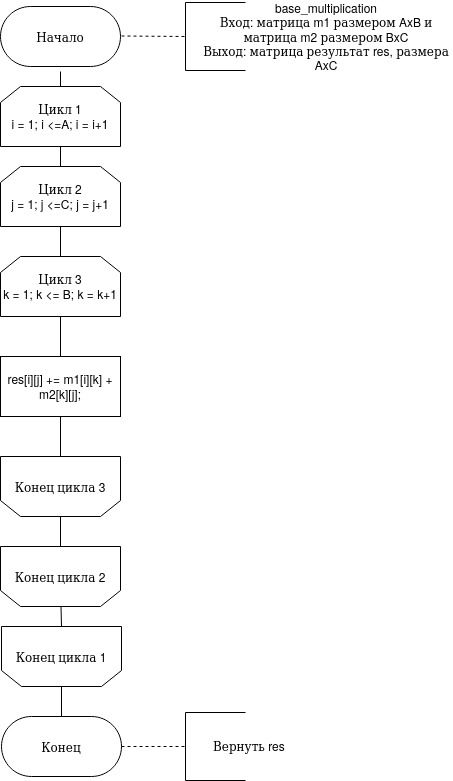
\includegraphics[width=1\linewidth]{base.jpg}
	\caption{Схема сортировки пузырьком}
	\label{fig:mpr}
\end{figure}

\begin{figure}[h]
	\centering
	%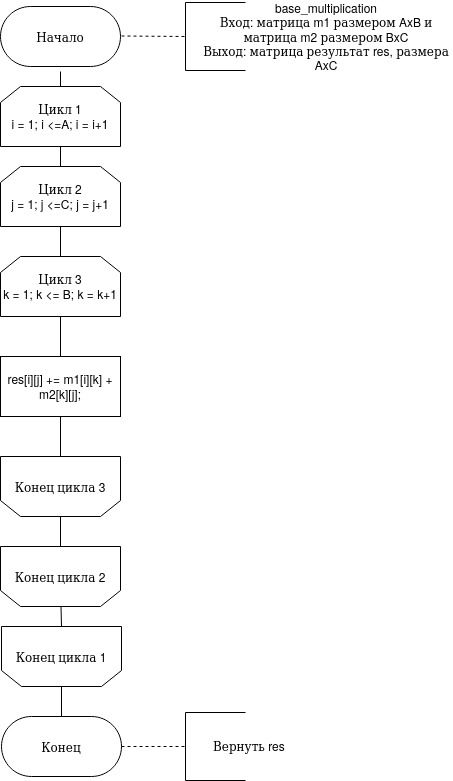
\includegraphics[width=1\linewidth]{base.jpg}
	\caption{Схема сортировки вставками}
	\label{fig:mpr}
\end{figure}

\begin{figure}[h]
	\centering
	%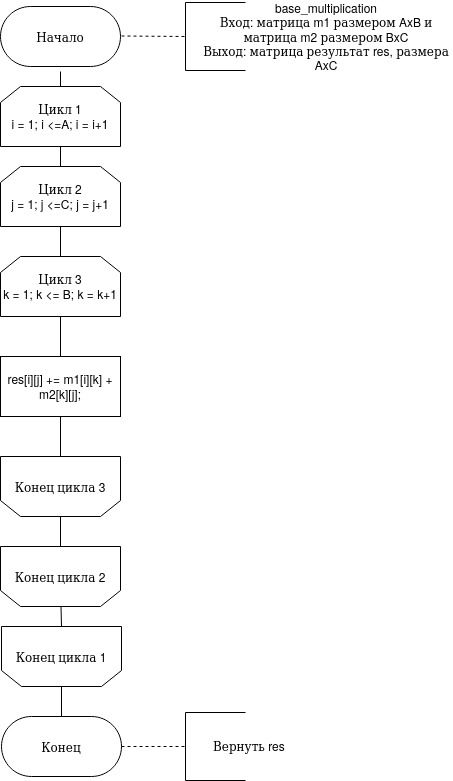
\includegraphics[width=1\linewidth]{base.jpg}
	\caption{Схема быстрой сортировки}
	\label{fig:mpr}
\end{figure}


\section{Модель вычислений}

Для последующего вычисления трудоемкости введём модель вычислений:

\begin{enumerate}
	\item Операции из списка (\ref{for:opers}) имеют трудоемкость 1.
	\begin{equation}
	\label{for:opers}
	+, -, /, \%, ==, !=, <, >, <=, >=, [], ++, {-}-
	\end{equation}
	\item Трудоемкость оператора выбора if условие then A else B рассчитывается, как (\ref{for:if}).
	\begin{equation}
	\label{for:if}
	f_{if} = f_{\text{условия}} +
	\begin{cases}
	f_A, & \text{если условие выполняется,}\\
	f_B, & \text{иначе.}
	\end{cases}
	\end{equation}
	\item Трудоемкость цикла рассчитывается, как (\ref{for:for}).
	\begin{equation}
	\label{for:for}
	f_{for} = f_{\text{инициализации}} + f_{\text{сравнения}} + N(f_{\text{тела}} + f_{\text{инкремента}} + f_{\text{сравнения}})
	\end{equation}
	\item Трудоемкость вызова функции равна 0.
\end{enumerate}

\section{Трудоёмкость алгоритмов}

Пусть размер массивов во всех вычислениях обозначается как $N$.

\subsection{Алгоритм сортировки пузырьком}

\subsection{Алгоритм сортировки вставками}

\section{Вывод}

На основе теоретических данных, полученных из аналитического раздела, были построены схемы трёх алгоритмов сортировки. Оценены их тредёмкости в лучшем и худшем случаях.

\chapter{Технологическая часть}

В данном разделе приведены средства реализации и листинги кода.

\section{Требование к ПО}

К программе предъявляется ряд требований:

\begin{itemize}
	\item На вход ПО получает массив сравнимых элементов;
	\item На выходе -- тот же массив, но отсортированный в заданном порядке.
\end{itemize}

\section{Средства реализации}
Для реализации ПО я выбрал язык программирования OCaml \cite{Ocaml}. Данный выбор обусловлен моим желанием расширить свои знания в области применения данного язкыа программирования. 

\section{Реализация алгоритмов}

В листингах 3.1 - 3.3 приведена реализация трёх алгоритмов сортировки.

\begin{lstlisting}[label=some-code,caption=Функция сортировки массива пузырьком, language=Caml]
let rec bsort arr =
  let rec _bsort = function
    | x1 :: x2 :: xs when x1 > x2 -> x2 :: _bsort (x1 :: xs)
    | x1 :: x2 :: xs -> x1 :: _bsort (x2 :: xs)
    | arr -> arr
  in
  let maybe_sorted = _bsort arr in
    if maybe_sorted = arr then arr
  else bsort maybe_sorted
;;
\end{lstlisting}

\begin{lstlisting}[label=some-code,caption=Функция сортировки массива вставками,language=Caml]
let rec isort arr =
  let rec insert k = function
    | x :: xs when k < x -> k :: x :: xs
    | x :: xs -> x :: (insert k xs)
    | arr -> [k]
  in
    match arr with
    | [] -> []
    | x :: xs -> insert x (isort xs)
;;
\end{lstlisting}

\begin{lstlisting}[label=some-code,caption=Функция быстрой сортировки,language=Caml]
let rec qsort = function
    | [] -> []
    | x :: xs -> let bot, top = List.partition (fun a -> a < x) xs
                 in qsort bot @ (x :: qsort top)
;;
\end{lstlisting}

\section{Тестовые данные}

В таблице~\ref{tbl:test} приведены тесты для функций, реализующих алгоритмы сортировки. Все тесты пройдены успешно.

\begin{table}[h!]
	\begin{center}
		\begin{tabular}{|c|c|c|}
			\hline
			Входной массив & Результат & Ожидаемый результат \\ 
			\hline
			$[15, 25, 35, 45, 55]$ & $[15, 25, 35, 45, 55]$  & $[15, 25, 35, 45, 55]$\\\hline
			$[55, 45, 35, 25, 15]$  & $[15, 25, 35, 45, 55]$ & $[15, 25, 35, 45, 55]$\\\hline
			$[-10, -20, -30, -25, -50]$  & $[-50, -30, -25, -20, -10]$  & $[-50, -30, -25, -20, -10]$\\\hline
			$[40, -10, 20, -30, 75]$  & $[-30, -10, 20, 40, 75]$  & $[-30, -10, 20, 40, 75]$\\\hline
			$[100]$  & $[100]$  & $[100]$\\\hline
			$[-20]$  & $[-20]$  & $[-20]$\\\hline
			Пустой массив  & Пустой массив  & Пустой массив\\
			\hline
		\end{tabular}
		\caption{\label{tbl:test}Тестирование функций}
	\end{center}
\end{table}

\section{Вывод}

В данном разделе были разработаны исходные коды трёх алгоритмов сортировки: пузырьком, вставками и быстрая сортировка.

\chapter{Исследовательская часть}

\section{Технические характеристики}

Ниже приведены технические характеристики устройства, на котором было проведено тестирование ПО:

\begin{itemize}
	\item Операционная система: Debian \cite{debian} Linux \cite{linux} 11 <<bullseye>> 64-bit.
	\item Оперативная память: 12 GB.
	\item Процессор: Intel(R) Core(TM) i5-3550 CPU @ 3.30GHz
\cite{i5}.

\end{itemize}

\section{Время выполнения алгоритмов}
Время выполнения алгоритм замерялось с помощью применения технологии профайлинга \cite{profiling}. Данный инстрмуент даёт детальное описание количества вызовов и количества времени CPU, занятого каждой функцией. \newline

\begin{table} [h!]
	\caption{Таблица времени выполнения сортировок на отсортированных данных (в секундах)}
	\begin{center}
		\begin{tabular}{|c c c c c|} 
			\hline
			Размер & Пузырьком & Вставками & Быстрая &\\  
			\hline
			100 & X & X & X &\\
			\hline
			200 & X & X & X &\\
			\hline
			300 & X & X & X &\\
			\hline
			500 & X & X & X &\\
			\hline
			1000 & X & X & X &\\
			\hline
			2500 & X & X & X &\\
			\hline
			5000 & X & X & X &\\
			\hline
			10000 & X & X & X &\\
			\hline
		\end{tabular}
	\end{center}
\end{table}

\begin{table} [h!]
	\caption{Таблица времени выполнения сортировок на отсортированных данных в обратном порядке (в секундах)}
	\begin{center}
		\begin{tabular}{|c c c c c|} 
			\hline
			Размер & Пузырьком & Вставками & Быстрая &\\  
			\hline
			100 & X & X & X &\\
			\hline
			200 & X & X & X &\\
			\hline
			300 & X & X & X &\\
			\hline
			500 & X & X & X &\\
			\hline
			1000 & X & X & X &\\
			\hline
			2500 & X & X & X &\\
			\hline
			5000 & X & X & X &\\
			\hline
			10000 & X & X & X &\\
			\hline
		\end{tabular}
	\end{center}
\end{table}

\begin{table} [h!]
	\caption{Таблица времени выполнения сортировок на случайных данных (в секундах)}
	\begin{center}
		\begin{tabular}{|c c c c c|} 
			\hline
			Размер & Пузырьком & Вставками & Быстрая &\\  
			\hline
			100 & X & X & X &\\
			\hline
			200 & X & X & X &\\
			\hline
			300 & X & X & X &\\
			\hline
			500 & X & X & X &\\
			\hline
			1000 & X & X & X &\\
			\hline
			2500 & X & X & X &\\
			\hline
			5000 & X & X & X &\\
			\hline
			10000 & X & X & X &\\
			\hline
		\end{tabular}
	\end{center}
\end{table}

\section{Вывод}

Тут какой то вывод..

\chapter*{Заключение}
\addcontentsline{toc}{chapter}{Заключение}

В рамках данной лабораторной работы:

\begin{enumerate}

	\item 123
\end{enumerate}



\addcontentsline{toc}{chapter}{Литература}

\bibliographystyle{utf8gost705u}  % стилевой файл для оформления по ГОСТу

\bibliography{51-biblio}          % имя библиографической базы (bib-файла)


\end{document}
